\selectlanguage{swedish}
\section{Polymerer}
%Grundläggande polymerkemi och vad som är gemensamt för allt inom materialgruppen och studien av polymerer.
Polymera material består utav polymer kedjor. Dessa kedjor är uppbyggda av repeteradne enheter av monomerer. Monomerer är den minsta repeterande enheten i en polymerkedja. Processen som kopplar samman monomerer till polymerkedjor är benämnd polymerisering.

\begin{figure}[ht]
    \centering
    % Träddiagram av polymertyperna:
%Ref: PolyT p. 5
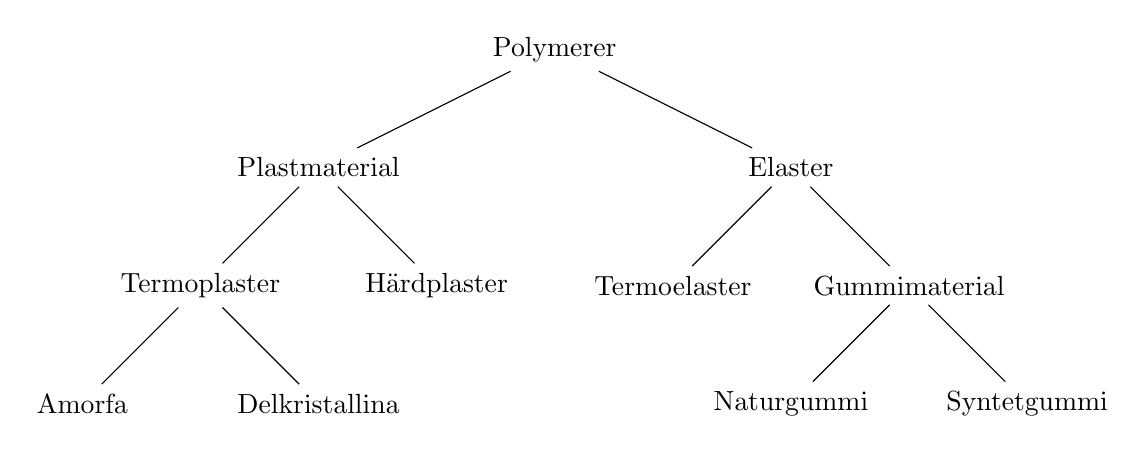
\begin{tikzpicture}[
    level 1/.style={sibling distance=6cm},
    level 2/.style={sibling distance=3cm},
    level 3/.style={sibling distance=3cm}
  ]
    \node {Polymerer}
        child { node {Plastmaterial}
            child { node {Termoplaster} 
                child { node {Amorfa} }
                child { node {Delkristallina} }    
            }
            child { node {Härdplaster} }
        }
        child { node {Elaster}
            child { node {Termoelaster} }
            child { node {Gummimaterial} 
                child { node {Naturgummi} }
                child { node {Syntetgummi} }
            }
        };
\end{tikzpicture}

    \caption{Kategorisering av polymertyper \cite[s.5]{polym}}
    \label{fig:polymer_typer}
\end{figure}

% %Beskrivning av skiljelinjen mellan plastmaterial och elaster.
% \subsection{Plaster}
% %Grundläggande om plastmaterial och deras egenskaper.
% \subsection{Elaster}
% %Grundläggande om elaster och deras egenskaper.

% \subsection{Naturliga polymerer}
% \subsection{Kommersiella polymerer}
% \subsection{Komposit material}

\subsection{Plaster och Elaster}
\subsubsection{Naturliga polymerer}
\subsubsection{Kommersiella polymerer}

\subsection{Molekylstrukturen}
\subsubsection{Molekylvikt}
\subsubsection{Konfiguration}
\subsubsection{Konformation}

\subsection{Mikrostrukturen}
%Amorf, delkristalina